\begin{frame}{Lien entre champ de repère 2D et maillage quadrilatère}
    \begin{center}
        \includegraphics[width=\linewidth]{img/quadsimu/singus.PNG}
        \small{
            \textit{Les singularités d'un champ de repère sont utilisées pour déterminer la position des sommets de valence différente de 4 dans le maillage quadrilatère.}
        }
    \end{center}
\end{frame}
\begin{frame}{Quadcover pour générer un maillage quadrilatère}
    \begin{center}
        \includegraphics[width=\linewidth]{img/cubecover/pipeline.PNG}
        \small{
            \textit{Les différentes étapes de la méthode Quadcover pour construire un maillage quadrilatère.}
        }
    \end{center}
\end{frame}
\begin{frame}{Les différents types de carte $U : \mathbb{R}^2 \mapsto \mathbb{R}^2$}
	\centering
	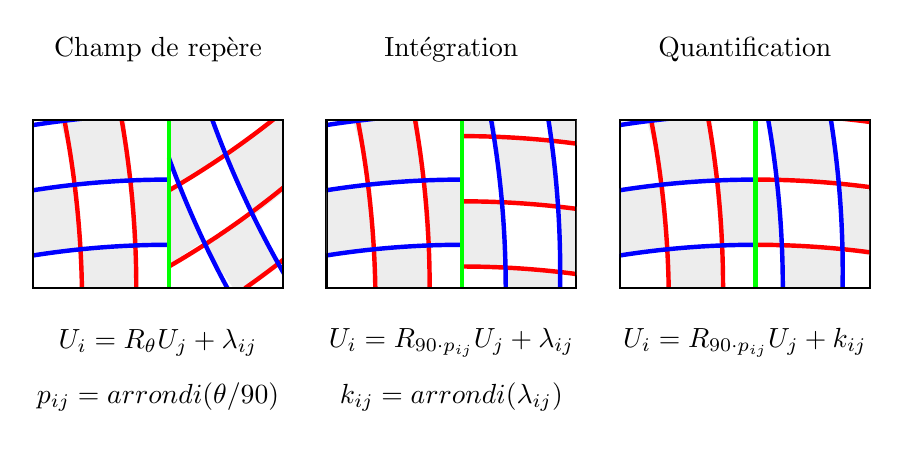
\begin{tikzpicture}[scale=1.38]
		\begin{scope}
			\draw[thick] (-.35, 0) -- (1.95, 0) -- (1.95, 1.55) -- (-.35, 1.55) -- cycle;
			\clip (-.35, 0) -- (1.95, 0) -- (1.95, 1.55) -- (-.35, 1.55) -- cycle;
			\fill[gray!14] (.06, .97) -- (.53, 1) -- (.5, 1.55) -- (-.1, 1.53);
			\fill[gray!14] (.06, .97) -- (-.5, .9) -- (-.5, .3) -- (.1, .37);
			\fill[gray!14] (.1, .37) -- (.57, .4) -- (.58, 0) -- (.1, 0);
			\fill[gray!14] (.57, .4) -- (.9, .4) -- (.9, 1.) -- (.53, 1.);
			\fill[gray!14] (.9, 1.2) -- (.9, 1.55) -- (1.3, 1.55) -- (1.44, 1.24) -- (.98, .96);
			\fill[gray!14] (1.44, 1.24) -- (1.95, 1.6) -- (1.95, .88) -- (1.68, .67);
			\fill[gray!14] (.9, .9) -- (.99, .98) -- (1.2, .42) -- (.9, .22);
			\fill[gray!14] (1.53, -.05) -- (1.2, .42) -- (1.68, .67) -- (1.9, .22);
			\draw[ultra thick, red] (0.1, 0) arc(1:11:9);
			\draw[ultra thick, red] (.6, 0) arc(0:10:9);
			\draw[ultra thick, blue] (.9, 0.4) arc(90:99:8);
			\draw[ultra thick, blue] (.9, 1) arc(90:99:8);
			\draw[ultra thick, blue] (.9, 1.6) arc(90:99:8);
			\draw[ultra thick, red] (.9, .2) arc(-60:-50:8);
			\draw[ultra thick, red] (.9, .9) arc(-60:-51:8);
			\draw[ultra thick, red] (1.6, 0) arc(-55:-51:8);
			\draw[ultra thick, blue] (.9, 1.2) arc(200:209:9);
			\draw[ultra thick, blue] (1.3, 1.55) arc(200:210:9);
			\draw[ultra thick, green] (.9, 0) -- (.9, 1.55);
			\draw[thick] (-.35, 0) -- (1.95, 0) -- (1.95, 1.55) -- (-.35, 1.55) -- cycle;
		\end{scope}
		\node at (.8, -0.5) {$U_i = R_{\theta} U_j + \lambda_{ij}$};
		\node at (.8, -1.) {$p_{ij} = arrondi(\theta/90)$};
		\node at (.8, 2.2) {Champ de repère};
		\begin{scope}[xshift=2.7cm]
			\draw[thick] (-.35, 0) -- (1.95, 0) -- (1.95, 1.55) -- (-.35, 1.55) -- cycle;
			\clip (-.35, 0) -- (1.95, 0) -- (1.95, 1.55) -- (-.35, 1.55) -- cycle;
			\fill[gray!14] (.06, .97) -- (.53, 1) -- (.5, 1.55) -- (-.1, 1.53);
			\fill[gray!14] (.06, .97) -- (-.5, .9) -- (-.5, .3) -- (.1, .37);
			\fill[gray!14] (.1, .37) -- (.57, .4) -- (.58, 0) -- (.1, 0);
			\fill[gray!14] (.57, .4) -- (.9, .4) -- (.9, 1.) -- (.53, 1.);
			\fill[gray!14] (.9, .2) -- (.9, .8) -- (1.27, .78) -- (1.29, .17);
			\fill[gray!14] (1.8, .16) -- (1.77, .76) -- (1.95, .75) -- (1.95, .12);
			\fill[gray!14] (1.27, .78) -- (1.77, .76) -- (1.74, 1.36) -- (1.22, 1.38);
			\fill[gray!14] (.9, 1.4) -- (1.22, 1.39) -- (1.2, 1.55) -- (.9, 1.55);
			\fill[gray!14] (1.73, 1.34) -- (1.71, 1.55) -- (1.95, 1.55) -- (1.95, 1.32);
			\fill[gray!14] (1.3, 0) -- (1.8, 0) -- (1.8, .14) -- (1.3, .18);
			\draw[ultra thick, red] (0.1, 0) arc(1:11:9);
			\draw[ultra thick, red] (.6, 0) arc(0:10:9);
			\draw[ultra thick, blue] (.9, 0.4) arc(90:99:8);
			\draw[ultra thick, blue] (.9, 1) arc(90:99:8);
			\draw[ultra thick, blue] (.9, 1.6) arc(90:99:8);
			\draw[ultra thick, red] (.9, .2) arc(90:82:8);
			\draw[ultra thick, red] (.9, .8) arc(90:82:8);
			\draw[ultra thick, red] (.9, 1.4) arc(90:82:8);
			\draw[ultra thick, blue] (1.3, 0) arc(0:10:9);
			\draw[ultra thick, blue] (1.8, 0) arc(-1:9:9);
			\draw[ultra thick, green] (.9, 0) -- (.9, 1.55);
			\draw[thick] (-.35, 0) -- (1.95, 0) -- (1.95, 1.55) -- (-.35, 1.55) -- cycle;
		\end{scope}
		\node at (3.5, -0.5) {$U_i = R_{90 \cdot p_{ij}} U_j + \lambda_{ij}$};
		\node at (3.5, -1.) {$k_{ij} = arrondi(\lambda_{ij})$};
		\node at (3.5, 2.2) {Intégration};
		\begin{scope}[xshift=5.4cm]
			\draw[thick] (-.35, 0) -- (1.95, 0) -- (1.95, 1.55) -- (-.35, 1.55) -- cycle;
			\clip (-.35, 0) -- (1.95, 0) -- (1.95, 1.55) -- (-.35, 1.55) -- cycle;
			\fill[gray!14] (.06, .97) -- (.53, 1) -- (.5, 1.55) -- (-.1, 1.53);
			\fill[gray!14] (.06, .97) -- (-.5, .9) -- (-.5, .3) -- (.1, .37);
			\fill[gray!14] (.1, .37) -- (.57, .4) -- (.58, 0) -- (.1, 0);
			\fill[gray!14] (.57, .4) -- (1.13, .4) -- (1.11, 1.) -- (.53, 1.);
			\fill[gray!14] (1.13, .4) -- (1.7, .36) -- (1.7, 0) -- (1.15, 0);
			\fill[gray!14] (1.11, 1.) -- (1.68, .96) -- (1.6, 1.55) -- (1.04, 1.55);
			\fill[gray!14] (1.68, .96) -- (1.95, .9) -- (1.95, .3) -- (1.7, .36);
			\draw[ultra thick, red] (0.1, 0) arc(1:11:9);
			\draw[ultra thick, red] (.6, 0) arc(0:10:9);
			\draw[ultra thick, blue] (.9, 0.4) arc(90:99:8);
			\draw[ultra thick, blue] (.9, 1) arc(90:99:8);
			\draw[ultra thick, blue] (.9, 1.6) arc(90:99:8);
			\draw[ultra thick, red] (.9, .4) arc(90:82:8);
			\draw[ultra thick, red] (.9, 1.) arc(90:82:8);
			\draw[ultra thick, red] (.9, 1.6) arc(90:80:8);
			\draw[ultra thick, blue] (1.15, 0) arc(0:10:9);
			\draw[ultra thick, blue] (1.7, 0) arc(-1:9:9);
			\draw[ultra thick, green] (.9, 0) -- (.9, 1.55);
			\draw[thick] (-.35, 0) -- (1.95, 0) -- (1.95, 1.55) -- (-.35, 1.55) -- cycle;
		\end{scope}
		\node at (6.2, -0.5) {$U_i = R_{90 \cdot p_{ij}} U_j + k_{ij}$};
		\node at (6.2, 2.2) {Quantification};
	
	\end{tikzpicture}
	
	%\caption{Classification des cartes en fonction de leur comportement à travers une discontinuité (en vert) : carte arbitraire (à gauche), carte sans couture (au milieu) et carte préservant la grille (à droite).}
	%\label{fig:all_diff_maps}
\end{frame}

\begin{frame}{En 3D: Cubecover pour générer un maillage hexaédrique}
    \begin{center}
        \includegraphics[width=\linewidth]{img/cubecover/B34_graphe_interieur.PNG}
        \small{
            \textit{Cubecover utilise le graphe de singularité d'un champ de repère 3D pour construire un maillage hexaédrique partageant le même graphe de singularité.}
        }
    \end{center}
\end{frame}